\section{Arbeitsablauf des Schlussfolgerers}

In der nachfolgenden Abbildung \ref{image-u2r3-workflow} ist der gewöhnliche Ablauf des Reasoner dargestellt. Dabei ist er in drei Hauptphasen einzuteilen. Das Laden der Ontologie, der Schlussfolgerungsvorgang und die Abfrage.

\begin{figure}[htp]
	\caption{Arbeitsablauf des Schlussfolgerers}
	\label{image-u2r3-workflow}
\begin{center}
	\scalebox{0.6}{
		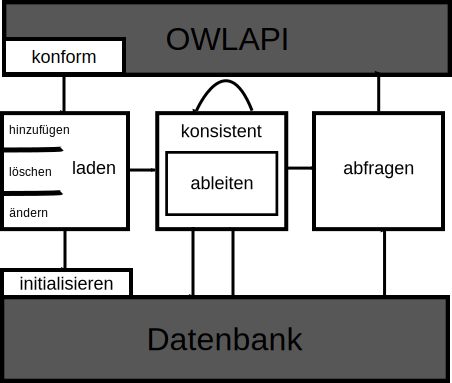
\includegraphics{images/u2r3-workflow.pdf}
	}
\end{center}
\end{figure}

Die sonstigen Bereich erledigen dabei das folgende:
\begin{itemize}
  \item Konformität: Dabei wird überprüft, ob die verwendete Syntax im OWL2 RL Profil liegt.
  \item Initialisierung: Hier wird falls notwendig das Datenbankschema erzeugt und Datenbankfunktionen werden eingerichtet.
\end{itemize}


\subsection{OWLAPI Anbindung}

Der obere Teil ist die sogenannte OWLAPI. Die OWLAPI ist eine Bibliothek die das Auslesen von Ontologien in verschiedenen Formaten erlaubt und eine Schlussfolgererschnittstelle für andere Programme zur Verfügung stellt. Durch die Implementierung dieser Schnittstelle in u2r3 ist es für alle Programme zugänglich die mit der OWLAPI arbeiten.
Die Schnittstelle stellt dabei auch eine Liste typischer Abfragen für einen Reasoner dar und kann allein dadurch schon als Messlatte für die Fähigkeiten eines Schlussfolgerers verwendet werden. Das OWLAPI-Projekt ist open-source und in Java implementiert und ist damit auch optimal für die Implementierung von u2r3 geeignet. Neben der reinen Parsertätigkeit kann die OWLAPI auch noch helfen zu überprüfen, ob eine Ontologie im OWL2 RL Profil liegt und nimmt damit weitere Arbeit ab.

\subsection{Das Laden einer Ontologie}
\label{abschnitt-laden-einer-ontologie}
Die Inhalte einer Ontolgie, die für das Schlussfolgern wichtig sind, sind die Axiome. Axiome sind dabei Fakten die als allgemein gültig angenommen werden. Sie dienen dazu das Universum der Ontologie zu modellieren und einen Startpunkt für weitere Schlussfolgerungen zu erzeugen.

Alle Axiome werden entsprechend dem MEMA-Prinzip abgelegt. Dabei ist für jedes Axiom genau eine Relation vorgesehen. Falls die Ontologie nicht OWL2 RL konform ist müssen für gewisse Axiome implizite Informationen abgelegt, wie. z.B. in der Regel \ref{rule-impl} zu sehen ist.

\begin{table}[htp]
	\caption{Eine implizite Regel}
	\label{rule-impl}
\begin{center}
	\begin{tabular}{l|l}
    If & then \\ \hline
	T(?i1, ?property, ?i2 ) & T(?property, owl:type, owl:ObjectProperty) \\
   \end{tabular}
\end{center}
\end{table}


Falls ein Axiom aus komplexen Ausdrücken zusammengesetzt ist werden die Ausdrücke rekursiv abgearbeitet und einzeln behandelt. Zum herstellen der Beziehungen bei komplexen Axiomen werden Platzhalter für die Ausdrücke verwendet. Die Platzhalter die dabei erzeugt werden stammen von der OWLAPI aus der NodeID Klasse und folgen damit dem selben Schema wie auch bei anonymen Individuen.

In folgendem Beispiel soll der komplexe Ausdruck $A \sqcap \exists p.B \sqsubseteq C$ abgespeichert werden. Zur Verdeutlichung wurden Klammern eingebaut.

\begin{equation}
\overbrace{
	(\overbrace{A \sqcap (
		\overbrace{\exists{}p.B}
		^{someValuesFrom(nid3, p, B) mit nid3:})}
	^{intersectionOf(nid1, nid2), list(nid2, A, nid3) mit nid2:})}
^{subClass(nid1, C) mit nid1:} \sqsubseteq C
\end{equation}
Wenn ein Ausdruck nicht direkt abgespeichert werden kann, dann wird für den Unterausdruck eine \emph{NodeID} erzeugt. Im obigen Beispiel werden drei Stück davon erzeugt. Diese stehen stellvertretend für den Unterausdruck. Es wird dann rekursiv weitergearbeitet bis alle in einfache Ausdrücke aufgelöst werden konnte.

Wenn Fakten in eine Relation geschrieben werden, wird von dieser ein Hinweis an den Regelprozessor geschickt neue Regelanwendungen in seine Warteschlange mitaufzunehmen. Der Hinweis an den Regelprozessor wird im folgenden oft auch als \emph{Reason} bezeichnet.
Der Regelprozessor überprüft diesen Hinweis und leitet daraus Regelanwendungen ab die er in einer Warteschleife abspeichert.

\subsection{Das Schlussfolgern in einer Ontologie}
Das Schlussfolgern in einer Ontologie besteht daraus die möglichen Regeln der OWL2 RL Spezifiaktion anzuwenden. Diese Regeln erzeugen neue Fakten oder überprüfen die Konsistenz. Der Schlussfolgerer hat seine Arbeit erledigt, wenn keine Regel neue Fakten erzeugen kann. Das sicherzustellen und dabei möglichst wenige Regeln anzuwenden ist seine Aufgabe. Daher wird im folgenden näher beschrieben, wann welche Regeln ausgelöst werden und in welcher Reihenfolge sie angewendet werden.

Die abzuarbeitenden Regeln enthalten eine Referenz auf die Fakten, die hinzugekommen sind. Allgemein sind sie so implementiert, das sie nur auf diesen neuen Fakten arbeiten -  auf den sogenannten Deltas - dies ist allerdings nicht in allen Fällen möglich (\emph{cls-int1}), sinnvoll (zu viele verschiedene Kombinationsmöglichkeiten) oder einfach zu komplex und damit fehleranfällig (\emph{prp-spo2}). Falls zwei oder mehrmals eine Regelanwendung auf die selben neuen Fakten erzeugt wird bevor sie ausgelöst wird, werden die beiden Regelanwendungen zu einer reduziert und können je nach Einstellung neu priorisiert werden.

All diese Regeln sind in einer Warteschleife abgelegt, die beim Laden der Ontologie gefüllt wird und beim Abarbeiten, d.h. dem Realisieren, der Ontologie ausgelesen wird.

Regeln können durch das Erzeugen von neuen Fakten Hinweise für den Regelprozessor geben der daraufhin weitere Regelanwendungen anlegt und in die Warteschlange einsortiert.

Der OWL2 RL Regelsatz garantiert dabei, das es immer zu einem Ende der Regelanwendung kommen wird, egal ob eine gültige oder ungültige Ontologie geladen wird.

\subsubsection{Auswertungsstrategien}
Die Auswertungstrategie beschreibt in welcher Reihenfolge der Regelprozessor die Anwendung von Regeln auslöst. 

Der naive Ansatz wäre alle Regeln nacheinander auszuführen, d.h. alle Regeln die implementiert sind anwenden, wenn eine der Regeln dabei neue Fakten erzeugt muss dieser Vorgang wiederholt werden. Dieses Vorgehen ist trotz seiner leichten Umsetzbarkeit nicht implementiert, da der Reasoner damit unnötig viel Arbeit verrichten müsste.

Ein etwas fortgeschrittener Ansatz ist es die Abhängigkeiten der Regeln auszunutzen, d.h. nur wenn für die Prämisse einer Regel überhaupt Fakten vorhanden sind kann diese ausgelöst werden. Das heißt im konkreten, wenn eine Relation die in einer Regel in der Prämisse verwendet wird neue Daten enthält, dann muss diese Regel ausgelöst werden. Dieses Verfahren ist im Schlussfolgerer so umgesetzt.

Es wurde allerdings diese Vorgehen noch etwas weiter verbessert. Veränderungen in verschiedenen Tabellen könnten mehrmals die selbe Regel auslösen, da die Regel mehrere Vorbedingungen  hat. Die Regel wird dann nicht mehrfach ausgelöst sondern es werden erst alle Regeln in eine Warteschlange gesammelt. Wird eine neue Regel ausgelöst, dann wird zuerst geschaut, ob diese Regel schon in der Warteschlange vorhanden ist.

Außerdem gibt es hier noch eine Optimierungsmöglichkeit, mit der man noch experimentieren kann. Wenn eine Regel in der Warteschlange erneut eingereiht werden soll, kann man sich entscheiden, ob die Regel an ihrere Stelle in der Schlange verbleibt oder ob sie herausgenommen wird und wieder ans Ende gestellt. Welches der beiden Verfahren besser ist muss sich erst noch in der Praxis zeigen.

In der Konfiguration des u2r3 ist diese Einstellungsmöglichkeit unter dem Namen \emph{EvaluationStrategy} zu finden. Gültige Werte dafür sind \emph{COMMONLAST} oder \emph{RARELAST}

\subsubsection{Regelauslösung}
Für jede Manipulation der Datenbank (Hinzufügung/Löschung) wird eine Reason ausgelöst. Es wird dabei nur eine Reason ausgelöst, egal wieviele Zeilen von der Manipulation betroffen waren. Eine Reason löst dann weitere Regelanwendungen aus, je nachdem welche Regeln davon betroffen sind [\ref{diagram-ruleexecution1}].

\begin{figure}[htp]
\begin{center}
\scalebox{0.75}{
  \begin{tikzpicture}[node distance=10em]
    \node[entity] (relation) {Relation};
    \node[relationship] (fireReason) [right of=relation] {löst aus}
        edge node[auto,swap] {1} (relation);
    \node[entity] (reason) [right of=fireReason] {Reason}
        edge node[auto,swap] {1} (fireReason);
    \node[relationship] (fireRuleAction) [right of=reason] {löst aus}
        edge node[auto,swap] {1} (reason);
    \node[entity] (ruleAction) [right of=fireRuleAction] {RuleAction}
        edge node[auto,swap] {k} (fireRuleAction);
\end{tikzpicture}
}
  \caption{Erzeugung der Regelanwendungen (Verhältnis)}
  \label{diagram-ruleexecution1}
\end{center}
\end{figure}

Bei der Erzeugung einer Reason sind dabei zwei Dinge wichtig. Das Delta, das sind die neuen Fakten und die Relation, da dort gespeichert ist welche Regeln auf die Relation angewendet werden können. Diese beiden Informationen ergeben eine Reason. Der Regelprozessor legt dann aus der Information in einer Reason evtl. mehrere Regelanwendungen in seiner Wartschleife an. Dieser Ablauf ist in Abb. \ref{diagram-ruleexecution2} dargestellt.

\begin{figure}[htp]
\begin{center}
	\scalebox{0.5}{
  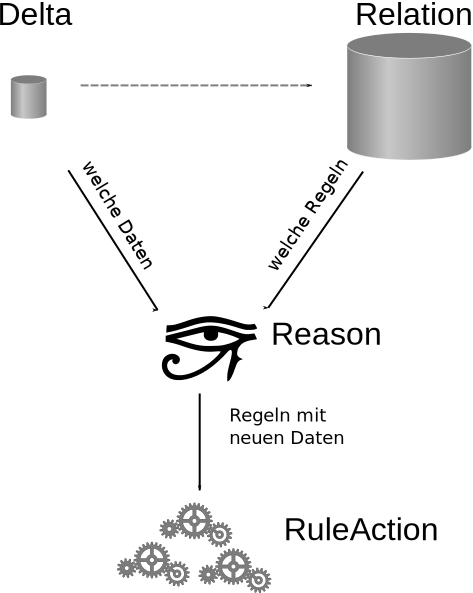
\includegraphics{images/regelausloesung.pdf}
	}
  \caption{Erzeugung der Regelanwendungen (Ablauf)}
  \label{diagram-ruleexecution2}
\end{center}
\end{figure}

\subsection{Das Abfragen einer Ontologie}
Das Abfragen in einer Ontologie lässt sich grundlegend in zwei Arten aufteilen. Erstens man hat einen Ausdruck und möchte überpürfen, ob dieser geschlussfolgert worden ist. Diese Art von Abfrage liefert nur ja oder nein zurück. Die zweite Art von Abfrage möchte eine Ergebnismenge zurück. Dabei ist im Gegensatz zur ersten Art von Abfrage eine Variable in der Abfrage, die gefüllt wird.

Bei beiden ist grundsätzlich so, dass das ``Anfrage'' OWL-Konstrukt in eine SQL-Abfrage umgeformt wird. In beiden Fällen kann die Abfrage beantwortet werden, egal ob die SQL-Abfrage etwas zurückbringt oder nicht. Im zweiten Fall muss aber bei einem Ergebnis daraus noch eine Ergebnis ereugt werden, so das es dem OWLAPI Format entspricht.

\subsubsection{Komplexe Ausdrücke finden}

Komplexe Ausdrücke sind OWL-Ausdrücke die sich aus einem oder mehr Unterausdrücken zusammensetzen. Für die Abspeicherung in u2r3 sind es alle Ausdrücke, die sich nicht direkt in eine Relation abspeichern lassen, sondern auf mehrere Relationen verteilen lässt. In der OWLAPI sind es alle Objekte, die keine eigene IRI haben.

Das Suchen nach einem komplexen Ausdruck gestaltet sich nicht so einfach wie vorher beschrieben, da die Abfrage nicht vollständig vorformliert werden kann, da die Unterausdrücke von unterschiedlicher Natur sind und auch die Tiefe und Verschachtelung der Ausdrücke nicht von vorneherein bekannt ist.

Als Lösung dafür kommen zwei Verfahren in Betracht. Erstens man führt einen neuen Namen für diesen komplexen Ausdruck ein. Dann muss über die Ontologie nocheinmal geschlossen werden, damit alle Zusammenhänge, die mit diesem komplexen Ausdruck verbunden sind auch mit diesem neuen Namen verbunden sind. Das ist alldergins sehr zeitaufwendig und zerstört den Vorteil dieses Reasoner, da alle Ergebnisse, die man Abfragen kann nach dem Schlussfolgern bereits in der Datenbank vorliegen. Außerdem verbaut man sich damit die Möglichkeit der Approximation beim Schlussfolgern. So muss nämlich erst komplett geschlussfolgert werden bevor eine Anfrage gestellt wird.

Darum ist das zweite Verfahren, das Aufbauen einer SQL-Abfrage. Diese kann dann zwar erst zur Laufzeit aufgebaut werden und ist schwerer für das RDBMS zu beantworten. Ein erneutes Schlussfolgern erübrigt sich aber. Das Aufbauen der SQL-Abfrage läuft dabei auch rekursiv ab. Die Unterausdrücke werden zu Unterabfragen in dem erstellten SQL-Ausdruck. Man setzt die Rekursion solange fort bis alle Unterausdrücke bei einfachen Ausdrücken angekommen sind.

Beim Zurückziehen von Fakten kann man das selbe Verfahren verwenden, um die komplexen Ausdrücke zu finden die man löschen möchte.